\section{Findings}
\label{sec:results}

\begin{table*}[t]
\centering
\caption{\textbf{Main benchmark} (test split, image-level AUC). Tasks are scored per edit family: injection (B-vs-C), removal (B-vs-D) and copy-move (A-vs-CM). For A-vs-B, 0.5 is ideal. FS is the fingerprint share (\cref{eq:fs}). Paired rows also see the null-twin reference (the lineage's LaMa twin), so they answer a different question from single-image rows, not the same one better. ``Paired control'' is trained on the paired model's rows but discards the reference. ``--'': not computed. Ranges summarise five published localisation checkpoints run zero-shot. AUCs alone do not rank these detectors; operating points are in \cref{tab:op}.}
\label{tab:main}
\footnotesize
\setlength{\tabcolsep}{4pt}
\begin{tabular}{@{}llccccccc@{}}
\toprule
 & Training & A-vs-C & B-vs-C & B-vs-D & A-vs-CM & A-vs-B (0.5) & FS & CT B-vs-C \\
\midrule
\multicolumn{9}{@{}l}{\emph{Synthetic-image detectors (single image)}}\\
AEROBLADE~\cite{ricker2024aeroblade} & none & 0.510 & 0.500$^{\S}$ & 0.50 & -- & -- & -- & -- \\ % src: Deepfakedoctillnow.pdf p.3; docs/council/context_dossier.md (B, E6 row)
NPR~\cite{tan2024npr} & A-vs-C & 0.502 & 0.500 & 0.501 & -- & -- & -- & 0.502 \\ % src: work/e0/out_local/tables/e6_baselines_v2.csv
UniFD~\cite{ojha2023unifd} & A-vs-C & 0.546 & 0.511 & 0.513 & -- & -- & -- & 0.507 \\ % src: work/e0/out_local/tables/e6_baselines_v2.csv
\midrule
\multicolumn{9}{@{}l}{\emph{Localisation models (single image)}}\\
Five checkpoints, zero-shot & external & 0.495--0.657 & 0.498--0.522 & 0.477--0.524 & 0.499--0.604 & 0.497--0.604 & -- & 0.501--0.512 \\ % src: work/e0/out_local/tables/table_main.csv (regime zeroshot)
IML-ViT~\cite{ma2023imlvit} (standard) & A-vs-C & 0.978 & 0.521 & 0.549 & 0.659 & 0.939 & 0.92 & 0.532 \\ % src: work/e0/out_local/tables/table_main.csv; FS: paper/data/fingerprint_share_test.csv
MVSS-Net~\cite{chen2021mvss} (standard) & A-vs-C & 0.721 & 0.539 & 0.534 & 0.534 & 0.677 & 0.80 & 0.509 \\ % src: work/e0/out_local/tables/table_main.csv; FS: paper/data/fingerprint_share_test.csv
TruFor~\cite{guillaro2023trufor} (standard) & A-vs-C & 0.688 & 0.520 & 0.522 & 0.624 & 0.628 & 0.68 & 0.516 \\ % src: work/e0/out_local/tables/table_main.csv; FS: paper/data/fingerprint_share_test.csv
Mesorch~\cite{zhu2025mesorch} (standard) & A-vs-C & 0.963 & 0.536 & 0.514 & 0.658 & 0.929 & 0.93 & 0.566 \\ % src: work/e0/out_local/tables/table_main.csv; FS: paper/data/fingerprint_share_test.csv
Mesorch + null-twin negatives & twins & 0.884 & 0.743 & 0.779 & 0.931 & 0.704 & 0.53 & 0.567 \\ % src: work/e0/out_local/tables/table_main.csv; FS: paper/data/fingerprint_share_test.csv
Mesorch + null-twin, distilled & twins & 0.918 & \textbf{0.768} & \textbf{0.870} & \textbf{0.932} & 0.668 & 0.40 & \textbf{0.586} \\ % src: work/e0/out_local/tables/e9_final_comparison.csv; B-vs-D, A-vs-CM, A-vs-B, FS: paper/data/main_benchmark_test.csv (derived)
Paired control, reference dropped & twins & 0.882 & 0.726 & 0.745 & 0.923 & 0.754 & 0.66 & 0.548 \\ % src: work/e0/out_local/tables/e3_table_bar.csv (pairnet_single); A-vs-C, A-vs-B, CT: paper/data/main_benchmark_test.csv (derived)
\midrule
\multicolumn{9}{@{}l}{\emph{Null-twin reference (paired)}}\\
Subtraction, 0 parameters & none & -- & 0.921 & 0.999 & 0.996 & -- & -- & 0.960 \\ % src: work/e0/out_local/e0x/e0a/E0A_REPORT.md
\quad standardised per modality & none & -- & 0.976 & -- & -- & -- & -- & 0.960 \\ % src: docs/council/round3/experiments/local/r3_subtraction_standardised.csv (standardised, ALL and ct)
Paired (FC-Siam-diff~\cite{daudt2018fcsiam})$^{\P}$ & twins & 0.992 & 0.984 & 0.996 & 0.988 & 0.498$^{\ast}$ & 0.00 & 0.927 \\ % src: work/e0/out_local/tables/e3_table_bar.csv; e9_final_comparison.csv; A-vs-B: paper/data/main_benchmark_test.csv (derived) = E3_REPORT.md 0.4976
\bottomrule
\end{tabular}\\[2pt]
\begin{minipage}{\linewidth}\footnotesize
$^{\S}$Copied from the programme summary; the summary table may have read the LaMa twin for this cell, which we will confirm (\TODO{re-pull AEROBLADE per-task CSV}).
$^{\P}$Post-selection: variants of this model family were revised after their test scores had been read, so the value is optimistic (\cref{sec:refverif}).
$^{\ast}$Twins of this kind were training negatives, so the value is in-distribution.
\end{minipage}
\end{table*}

\subsection{Detectors respond to the autoencoder, not the edit}
\label{sec:confound}

\Cref{tab:main} gives the main benchmark.
Every conventionally fine-tuned localisation model collapses when its negatives become null twins.
Mesorch falls from 0.963 on A-vs-C to 0.536 on B-vs-C, % src: work/e0/out_local/tables/table_main.csv
and IML-ViT from 0.978 to 0.521. % src: work/e0/out_local/tables/table_main.csv
Their fingerprint shares are 0.93 and 0.92: almost all of the margin they report is reproduced by an image nobody edited. % src: paper/data/fingerprint_share_test.csv (derived); work/e0/out_local/tables/E1_REPORT.md
Across the four fine-tuned models that learned the task, FS ranges from 0.68 to 0.93. % src: work/e0/out_local/tables/E1_REPORT.md (fp share table)
Published checkpoints run zero-shot and the synthetic-image detectors sit near chance on the twin-controlled tasks (B-vs-C between 0.498 and 0.522) % src: work/e0/out_local/tables/table_main.csv; work/e0/out_local/tables/e6_baselines_v2.csv
and are weak even on A-vs-C (at most 0.657), % src: work/e0/out_local/tables/table_main.csv (trufor zeroshot)
as expected for whole-image methods facing edits that cover 0.1--5\% of the frame; % src: Deepfakedoctillnow.pdf p.2
we report them as methods applied outside their design regime, and NPR and UniFD were fitted on only 4,619 training images. % src: Deepfakedoctillnow.pdf p.9

\begin{table}[t]
\centering
\caption{\textbf{The autoencoder response on MedForge.} AUC of each image type against the untouched MedForge test scans (0.5: indistinguishable from untouched), and the Reasoner's hard ``deepfake'' rate. No pixel is edited in the JPEG, SD and SDXL columns. Mesorch rows exclude 25 brain-MRI scans that duplicate our sources. % src: docs/council/round2/experiments/README.md (Step 9, job A)
Chest X-ray is not evaluated (credentialed access).}
\label{tab:medforge}
\footnotesize
\setlength{\tabcolsep}{3.5pt}
\begin{tabular}{@{}lcccc@{}}
\toprule
 & \multicolumn{3}{c}{unedited scan passed through} & \multirow{2}{*}{\shortstack{MedForge\\forgery}} \\
\cmidrule(lr){2-4}
Scorer (scans) & JPEG q95 & SD AE & SDXL AE & \\
\midrule
MedForge-Reasoner, AUC & 0.500 & \textbf{0.960} & 0.858 & 0.997 \\ % src: work/e0/out_local/e2/e2_table.csv
\quad flagged, brain MRI (untouched 1.0\%) & 1.0\% & \textbf{95.8\%} & 65.6\% & 100\% \\ % src: docs/council/round3/experiments/local/r3_box_audit.csv (brain-mri, fake_rate)
\quad flagged, fundus (untouched 0.0\%) & 0.0\% & \textbf{88.9\%} & 78.9\% & 100\% \\ % src: docs/council/round3/experiments/local/r3_box_audit.csv (fundus, fake_rate)
\quad PSNR to untouched (dB) & 57.5--64.6 & 38.1--39.5 & -- & -- \\ % src: docs/council/round3/experiments/local/r3_chairman_crosscheck.csv (per-modality medians)
Mesorch, standard & 0.497 & 0.666 & 0.613 & 0.521 \\ % src: work/e0/out_local/e2/e2_table.csv
\quad brain MRI & 0.489 & \textbf{0.842} & 0.731 & -- \\ % src: work/e0/out_local/e2/e2_table.csv
Mesorch + null twins & 0.497 & 0.523 & 0.516 & 0.555 \\ % src: work/e0/out_local/e2/e2_table.csv
\quad brain MRI & 0.498 & \textbf{0.575} & 0.563 & -- \\ % src: work/e0/out_local/e2/e2_table.csv
\bottomrule
\end{tabular}
\end{table}

\begin{figure*}[t]
\centering
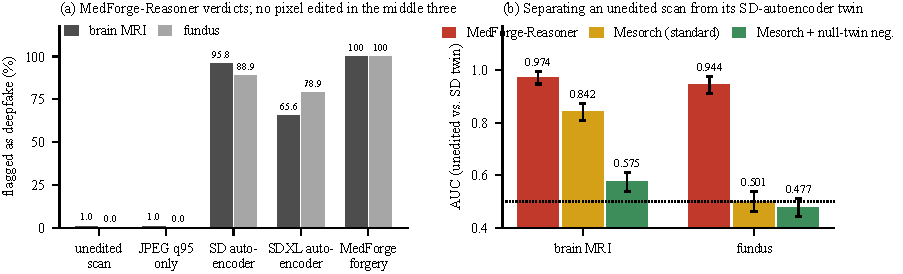
\includegraphics[width=0.98\linewidth]{figures/fig_medforge.pdf}
\caption{\textbf{MedForge's own detector responds to the autoencoder.} (a) MedForge-Reasoner's ``deepfake'' verdicts per modality on 96 brain-MRI and 90 fundus untouched MedForge test scans, % src: docs/council/round3/experiments/local/r3_box_audit.csv (n per arm)
the same scans after JPEG re-encoding or an autoencoder round trip with no edit, and 48 MedForge forgeries. % src: paper/data/medforge_reasoner_hardlabel.csv
(b) AUC separating an untouched scan from its SD-autoencoder twin, with 95\% intervals. Standard Mesorch responds to the twin on brain MRI, which it was trained on, but not on fundus, which it has never seen. Values await confirmation on a fresh sample (\TODO{E3b: fresh sample}).}
\label{fig:medforge}
\end{figure*}

\paragraph{MedForge.}
To test whether the response is an artefact of our own pipeline, we sampled untouched scans from MedForge-90K's test split (brain MRI and fundus) and built three versions that edit nothing: a JPEG re-save at quality 95, which is how MedForge stores its forgeries, % src: docs/council/round2/experiments/README.md (harness fact 6); E2_medforge_confound.md (JPEG step)
and SD- and SDXL-autoencoder round trips followed by the same JPEG step.
MedForge-Reasoner~\cite{chen2026medforge}, an 8B vision-language detector, % src: docs/council/round2/landscape_and_odds.md (Sec. 1)
flags all 48 forgeries we sampled and 1 of 186 untouched scans (\cref{tab:medforge,fig:medforge}). % src: paper/data/medforge_reasoner_hardlabel.csv
After an SD-autoencoder round trip it flags 95.8\% of brain MRI and 88.9\% of fundus scans, % src: docs/council/round3/experiments/local/r3_box_audit.csv (N_sd, real)
and after an SDXL round trip 65.6\% and 78.9\%. % src: docs/council/round3/experiments/local/r3_box_audit.csv (N_sdxl, real)
Its fingerprint share is 0.92 for the SD round trip and 0.72 for SDXL. % src: paper/data/medforge_fingerprint_share.json (derived from work/e0/out_local/e2/e2_table.csv)
The verdicts are localised.
Every one of its 306 ``deepfake'' calls on an unedited round trip comes with a box, and no ``real'' call does; % src: docs/council/round3/experiments/local/R3_STEP1_REPORT.md (Sec. 1)
the median box covers 2.0\% of a brain scan and 3.9\% of a fundus image, % src: docs/council/round3/experiments/local/r3_box_audit.csv (N_sd, real, area_median)
against 3.6\% and 2.3\% for its boxes on real MedForge forgeries. % src: docs/council/round3/experiments/local/r3_box_audit.csv (R, forged, area_median)
On 22 of the 30 sampled scans labelled normal (12 of 16 brains), it reports a localised manipulation after the SD round trip, % src: docs/council/round3/experiments/local/r3_box_audit_normals.csv (N_sd)
and for the same source its SD and SDXL boxes overlap with a median IoU of 0.83 (133 sources; 0.056 for shuffled sources), % src: docs/council/round3/experiments/local/R3_STEP1_REPORT.md (Sec. 1); r3_chairman_crosscheck.csv
so the box follows the image content rather than a fixed prior location: the Reasoner describes a lesion-sized edit that does not exist.
The JPEG version scores 0.500, % src: work/e0/out_local/e2/e2_table.csv
but it is a far milder change (57.5--64.6\,dB PSNR to the untouched scan, against 38.1--39.5\,dB for the SD round trip), % src: docs/council/round3/experiments/local/r3_chairman_crosscheck.csv (per-modality medians)
so it does not show that non-neural processing of the same strength would pass. \TODO{E3b: JPEG, JPEG 2000 and a learned codec at the SD round trip's PSNR; local SD null; fresh sample}
Standard Mesorch, trained only on our data, shows the same response on MedForge brain MRI (0.842) % src: work/e0/out_local/e2/e2_table.csv
and none on fundus (0.501), a modality it has never seen; % src: work/e0/out_local/e2/e2_table.csv
twin negatives cut it to 0.575, % src: work/e0/out_local/e2/e2_table.csv
although neither Mesorch variant detects MedForge's own forgeries (0.521 and 0.555). % src: work/e0/out_local/e2/e2_table.csv

\paragraph{A held-out generator, and twin training.}
The same response appears with SDXL, which no model saw in training: standard Mesorch separates untouched sources from their SDXL twins at 0.842, % src: docs/council/round2/experiments/README.md (Step 5)
twin-trained Mesorch at 0.601. % src: docs/council/round2/experiments/README.md (Step 5)
Training Mesorch with twins as negatives lifts B-vs-C from 0.536 to 0.743, % src: work/e0/out_local/tables/table_main.csv
and distillation from the paired model to 0.768. % src: work/e0/out_local/tables/e9_final_comparison.csv
The gain is specific to the backbone: of five backbones trained the same way, only Mesorch gains more than 0.10 (MVSS-Net $+$0.023, TruFor $-$0.010). % src: work/e0/out_local/tables/E2_REPORT.md (Step 1)
It does not reach CT, which stays at 0.567, % src: work/e0/out_local/tables/table_main.csv
and it leaves a residual false alarm, A-vs-B 0.704 (\cref{sec:shortcuts}). % src: work/e0/out_local/tables/table_main.csv

\subsection{Operating points: no detector wins everywhere}
\label{sec:operating}

\begin{table*}[t]
\centering
\caption{\textbf{Operating points.} One threshold per detector, fixed at 95\% TPR on calibration SD injections pooled over modalities; every rate is read at that threshold. Cells give pooled\,/\,CT, in \%. Rates are on calibration except ``SD twin, test''; rows marked $^{\ddagger}$ are on test throughout, because their calibration scores are not stored locally. $^{\circ}$Held out of training for the last three rows; no other row saw any benign operation. ``SDXL twin'': FPR on calibration SDXL twins\,/\,on SD twins matched to them on in-mask MSE ($\star$: pending, \TODO{E3a: SDXL holdout and MSE-matched SD nulls}); not computed for CT. ``worst'': maximum FPR over the calibration SD twins (test for $^{\ddagger}$ rows), untouched sources and the four benign operations. AE: autoencoder round trip of the whole source. Per-modality rows are in the supplementary material.}
\label{tab:op}
\footnotesize
\setlength{\tabcolsep}{2.3pt}
\begin{tabular}{@{}lcccccccccc@{}}
\toprule
 & & \multicolumn{2}{c}{SD twin} & & \multicolumn{4}{c}{benign operation on the source} & & \\
\cmidrule(lr){3-4}\cmidrule(lr){6-9}
Detector & TPR & cal. & test & untouched & JPEG & VQ-AE & NL-means$^{\circ}$ & SDXL-AE$^{\circ}$ & SDXL twin & worst \\
\midrule
\multicolumn{11}{@{}l}{\emph{Single image (Mesorch)}}\\
standard & 94.9\,/\,72.6 & 93.3\,/\,68.4 & 95.2\,/\,78.5 & 35.0\,/\,63.2 & 32.8\,/\,63.2 & 53.6\,/\,71.4 & 64.4\,/\,74.6 & 47.9\,/\,65.4 & 82.9\,/\,$\star$ & 93.3\,/\,74.6 \\ % src: docs/council/round3/experiments/local/r3_operating_points.csv (V0, ALL / ct); SDXL twin: R3_STEP1_REPORT.md Sec. 4 (E0e, carried over)
+ null twins & 94.9\,/\,72.6 & 94.0\,/\,70.5 & 95.6\,/\,73.6 & 84.1\,/\,66.5 & 89.2\,/\,84.9 & 87.5\,/\,69.7 & 94.9\,/\,87.6 & 84.1\,/\,68.6 & 90.9\,/\,$\star$ & 94.9\,/\,87.6 \\ % src: docs/council/round3/experiments/local/r3_operating_points.csv (V1, ALL / ct); SDXL twin: R3_STEP1_REPORT.md Sec. 4 (E0e)
+ distilled$^{\ddagger}$ & 95.9\,/\,91.7 & -- & 72.3\,/\,89.3 & 41.2\,/\,87.4 & 38.1\,/\,73.6 & 48.0\,/\,87.0 & 54.0\,/\,82.1 & 40.2\,/\,83.3 & 61.3\,/\,$\star$ & 72.3\,/\,89.3 \\ % src: docs/council/round3/experiments/local/r3_operating_points.csv (V1d, ALL / ct, test, tpr_test_C_sd); SDXL twin: R3_STEP1_REPORT.md Sec. 4 (E0e)
\midrule
\multicolumn{11}{@{}l}{\emph{Null-twin reference}}\\
subtraction & 94.9\,/\,91.6 & 43.8\,/\,14.7 & 46.7\,/\,12.4 & 12.0\,/\,2.7 & 15.3\,/\,4.3 & 99.3\,/\,100 & 26.3\,/\,41.1 & 98.4\,/\,100 & $\star$ & 99.3\,/\,100 \\ % src: docs/council/round3/experiments/local/r3_operating_points.csv (sub_raw, ALL / ct)
\quad standardised & 94.9\,/\,91.6 & 14.9\,/\,14.7 & 12.1\,/\,11.6 & 1.0\,/\,2.7 & 4.1\,/\,4.3 & 72.5\,/\,100 & 21.0\,/\,38.9 & 83.9\,/\,100 & $\star$ & 83.9\,/\,100 \\ % src: docs/council/round3/experiments/local/r3_operating_points.csv (sub_std, ALL / ct)
paired (FC-Siam-diff)$^{\ddagger}$ & 97.0\,/\,86.0 & -- & 13.6\,/\,5.8 & 1.7\,/\,0.0 & 19.6\,/\,41.1 & 38.4\,/\,91.5 & 78.4\,/\,98.8 & 70.6\,/\,96.7 & 5.5\,/\,$\star$ & 78.4\,/\,98.8 \\ % src: docs/council/round3/experiments/local/r3_operating_points.csv (p1n, ALL / ct, test, tpr_test_C_sd); SDXL twin: R3_STEP1_REPORT.md Sec. 4 (E0e)
+ benign negatives & 94.9\,/\,77.9 & 11.1\,/\,4.2 & 10.1\,/\,1.7 & 0.2\,/\,0.0 & 0.5\,/\,0.0 & 10.1\,/\,25.4 & 11.8\,/\,8.1 & 26.9\,/\,52.4 & $\star$ & 26.9\,/\,52.4 \\ % src: docs/council/round3/experiments/local/r3_operating_points.csv (p2, ALL / ct)
\quad + invariance, $\lambda$=0.03 & 94.9\,/\,80.0 & 6.0\,/\,7.4 & 6.1\,/\,3.3 & 0.1\,/\,0.0 & 0.0\,/\,0.0 & 4.3\,/\,9.7 & 1.5\,/\,0.0 & 8.8\,/\,20.5 & $\star$ & \textbf{8.8}\,/\,\textbf{20.5} \\ % src: docs/council/round3/experiments/local/r3_operating_points.csv (p3_0.03, ALL / ct)
\quad + invariance, $\lambda$=0.1 & 94.9\,/\,78.9 & 27.8\,/\,60.0 & 29.0\,/\,62.0 & 18.2\,/\,8.6 & 8.8\,/\,0.5 & 24.2\,/\,33.0 & 12.9\,/\,10.3 & 26.3\,/\,32.4 & $\star$ & 27.8\,/\,60.0 \\ % src: docs/council/round3/experiments/local/r3_operating_points.csv (p3_0.1, ALL / ct)
\bottomrule
\end{tabular}
\end{table*}

\begin{figure}[t]
\centering
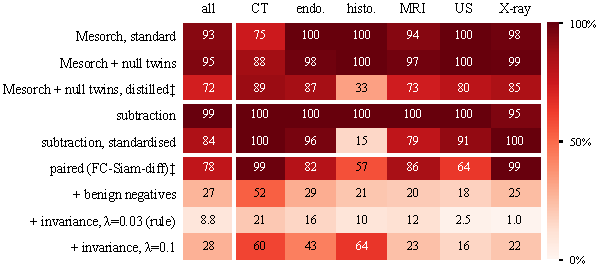
\includegraphics[width=\linewidth]{figures/fig_operating.pdf}
\caption{\textbf{Worst false-positive rate per modality} (\%), over SD twins, untouched sources and four benign operations, at each detector's pooled calibration threshold (95\% TPR on SD injections). Rows as in \cref{tab:op}; $^{\ddagger}$test-split rates. No row is light in every column.}
\label{fig:operating}
\end{figure}

\Cref{tab:op,fig:operating} put every Mesorch-based and reference-based detector at one threshold and read it against each negative type.
No detector wins everywhere, and a high AUC does not imply a usable operating point.
Fine-tuned single-image detectors flag 93.3\% (standard) and 94.0\% (twin-trained) of calibration SD twins, % src: docs/council/round3/experiments/local/r3_operating_points.csv (V0, V1, fpr_cal_SD_null)
so their AUC margins carry no alarm rate a user could live with.
Subtraction, at AUC 0.921, flags 43.8\% of calibration and 46.7\% of test SD twins, % src: docs/council/round3/experiments/local/r3_operating_points.csv (sub_raw, fpr_cal_SD_null, fpr_test_SD_null)
and 99.3\% and 98.4\% of sources round-tripped through the VQ and SDXL autoencoders. % src: docs/council/round3/experiments/local/r3_operating_points.csv (sub_raw, fpr_vqvae, fpr_sdxlvae)
Standardising it per modality lifts its AUC to 0.976 % src: docs/council/round3/experiments/local/r3_subtraction_standardised.csv (standardised, ALL)
but still flags 72.5\% and 83.9\% of those round trips, % src: docs/council/round3/experiments/local/r3_operating_points.csv (sub_std, fpr_vqvae, fpr_sdxlvae)
and all of them on CT.
The paired baseline flags 13.6\% of test SD twins, % src: docs/council/round3/experiments/local/r3_operating_points.csv (p1n, fpr_test_SD_null)
but 78.4\% of denoised and 70.6\% of SDXL-autoencoded sources (98.8\% and 96.7\% on CT). % src: docs/council/round3/experiments/local/r3_operating_points.csv (p1n, fpr_nlmeans, fpr_sdxlvae, ALL / ct)
On CT every detector is weaker at the pooled threshold; single-image Mesorch recalls 72.6\% of injections. % src: docs/council/round3/experiments/local/r3_operating_points.csv (V0, V1, ct, tpr_cal_C_sd)

\paragraph{Drift beside transfer.}
Thresholds drift even without a change of generator: the twin-trained model's SD-twin FPR moves from 94.0\% on calibration to 95.6\% on test, and subtraction's from 43.8\% to 46.7\%. % src: docs/council/round3/experiments/local/r3_operating_points.csv (V1, sub_raw: fpr_cal_SD_null, fpr_test_SD_null)
A raw cross-generator rate is not comparable with these: the paired baseline flags 5.5\% of SDXL twins, less than the 13.6\% it flags on SD twins, % src: docs/council/round3/experiments/local/R3_STEP1_REPORT.md (Sec. 4, E0e carried over); r3_operating_points.csv (p1n, fpr_test_SD_null)
because an SDXL twin sits about 7$\times$ closer to its source (in-mask MSE 1.83 against 13.54) and is an easier negative. % src: docs/council/round2/experiments/README.md (Step 5)
Transfer is therefore read against SD twins matched on in-mask MSE (\TODO{E3a: MSE-matched SD-null FPR}).

\paragraph{AUC and operating-point selection disagree.}
For the paired baseline with an invariance penalty, choosing $\lambda$ by how little the output changes under benign processing picks $\lambda=0.1$; % src: round3/council_verdict.md (pending r3_step1) (Where the Council Clashes: lambda=0.1 was chosen by AUC deviation)
at its threshold that model flags 18.2\% of untouched calibration sources (20.2\% on test) and 27.8\% of SD twins. % src: docs/council/round3/experiments/local/r3_operating_points.csv (p3_0.1: fpr_A, fpr_A_test, fpr_cal_SD_null)
Our pre-registered rule (\cref{sec:protocol}) picks $\lambda=0.03$ instead, whose worst calibration FPR over the five selection negatives is 6.0\%, against 11.8\% without the penalty and 27.8\% and 43.3\% for $\lambda=0.1$ and 0.3. % src: docs/council/round3/experiments/local/r3_lambda_preregistration.json (max_fpr)

\subsection{Reference-verification baselines}
\label{sec:refverif}

\begin{table}[t]
\centering
\caption{\textbf{Reference-verification baselines} (test AUC). All use the null-twin reference. ``worst FPR'': pooled\,/\,CT, in \%, from \cref{tab:op}. $^{\P}$Post-selection on test (see text). $^{\ddagger}$Test-split rates.}
\label{tab:refverif}
\footnotesize
\setlength{\tabcolsep}{3pt}
\begin{tabular}{@{}lcccc@{}}
\toprule
Baseline & B-vs-C & CT & B-vs-D & worst FPR \\
\midrule
subtraction, 0 parameters & 0.921 & \textbf{0.960} & \textbf{0.999} & 99.3\,/\,100 \\ % src: work/e0/out_local/e0x/e0a/E0A_REPORT.md; worst FPR: docs/council/round3/experiments/local/r3_operating_points.csv (sub_raw)
\quad standardised & 0.976 & \textbf{0.960} & -- & 83.9\,/\,100 \\ % src: docs/council/round3/experiments/local/r3_subtraction_standardised.csv; r3_operating_points.csv (sub_std)
block-wise robust hash & \multicolumn{4}{c}{\PENDING{E3c}} \\
paired (FC-Siam-diff)$^{\P}$ & \textbf{0.984} & 0.927 & 0.996 & 78.4\,/\,98.8$^{\ddagger}$ \\ % src: paper/data/paired_family_test_auc.csv (derived); r3_operating_points.csv (p1n)
\quad + benign negatives$^{\P}$ & 0.978 & 0.952 & 0.994 & 26.9\,/\,52.4 \\ % src: paper/data/paired_family_test_auc.csv (derived, p2); docs/council/round3/experiments/local/r3_operating_points.csv (p2)
\quad\quad + invariance, $\lambda$=0.03$^{\P}$ & 0.982 & 0.934 & 0.997 & \textbf{8.8}\,/\,\textbf{20.5} \\ % src: paper/data/paired_family_test_auc.csv (derived, p3 lam=0.03); docs/council/round3/experiments/local/r3_operating_points.csv (p3_0.03)
\bottomrule
\end{tabular}
\end{table}

When a reference image is available, detection becomes verification against it (\cref{tab:refverif}).
Every row here uses the null-twin reference, not a pristine original; rescoring with the source as reference is pending (\TODO{E3a: pristine-reference rescoring}).
A zero-parameter subtraction reaches 0.921 [0.910, 0.931] on B-vs-C, % src: docs/council/round3/experiments/local/r3_subtraction_standardised.csv (raw, ALL)
and 0.976 [0.968, 0.982] once its score is standardised per modality on calibration twins. % src: docs/council/round3/experiments/local/r3_subtraction_standardised.csv (standardised, ALL)
Telling it the true mask adds nothing (0.9208 against 0.9210), % src: work/e0/out_local/e0x/e0a/E0A_REPORT.md
whereas a byte-level hash is at chance (0.506), % src: work/e0/out_local/e0x/e0a/E0A_REPORT.md
because every image differs from the reference across the whole feather.
The paired model's control, trained on identical rows without the reference, scores 0.726, % src: work/e0/out_local/tables/e3_table_bar.csv (pairnet_single)
so the reference is what makes the task easy, and any claim that \dataset is hard must read ``hard without a reference''.

The paired baseline, FC-Siam-diff on a Mesorch trunk with the LaMa null twin as reference, reaches 0.984. % src: work/e0/out_local/tables/e3_table_bar.csv
This number is post-selection: variants of this paired model family were revised after their test scores had been read, so it is optimistic. % src: docs/council/round3/council_verdict.md (Blind Spots: the test split is spent for PAIR-NET-family claims)
Its margin over raw subtraction, $+$0.063 [0.053, 0.073], % src: docs/council/round3/experiments/local/r3_subtraction_gap_to_p1n.csv (raw, ALL)
shrinks to $+$0.008 [0.001, 0.016] over standardised subtraction, % src: docs/council/round3/experiments/local/r3_subtraction_gap_to_p1n.csv (standardised, ALL)
so almost all of it is per-modality calibration.
Per modality, the paired baseline still leads on endoscopy ($+$0.074) and trails on CT ($-$0.033). % src: docs/council/round3/experiments/local/r3_subtraction_gap_to_p1n.csv (standardised, endoscopy, ct)
At its operating point it does not separate an edit from benign reprocessing either (\cref{tab:op}).

Adding JPEG and VQ-autoencoder copies of sources as negatives, and then an output-invariance penalty, changes the operating point far more than the AUC.
Of the detectors tested, only a reference-paired verifier trained with benign negatives and an output-invariance penalty keeps FPR under 10\% on every negative type at one threshold; we report it as a baseline. % src: docs/council/round3/experiments/local/r3_operating_points.csv (p3_0.03, ALL, worst_fpr 0.088)
\PENDING{Pending E3a (pristine-reference rescoring and SDXL holdout).}
The statement is pooled over modalities, where its worst rate is 8.8\%, on the held-out SDXL autoencoder; % src: docs/council/round3/experiments/local/r3_operating_points.csv (p3_0.03, ALL, worst_fpr_on fpr_sdxlvae)
its SD-twin rate barely drifts (6.0\% on calibration, 6.1\% on test). % src: docs/council/round3/experiments/local/r3_operating_points.csv (p3_0.03, fpr_cal_SD_null, fpr_test_SD_null)
$\lambda=0.03$ was set by the min--max calibration FPR rule, written down before any SDXL score was read; the rule is not blind, since its calibration inputs had been inspected, but it locks the choice before the held-out generator and further seeds are scored. % src: docs/council/round3/experiments/local/r3_lambda_preregistration.json (honesty_note)
Its B-vs-C AUC of 0.982 is within 0.01 of standardised subtraction, so we make no AUC claim for it. % src: paper/data/paired_family_test_auc.csv (derived, p3 lam=0.03, b_vs_c)
On CT it is weak: it flags 20.5\% of SDXL-autoencoded scans and recalls 80.0\% of injections at the pooled threshold, % src: docs/council/round3/experiments/local/r3_operating_points.csv (p3_0.03, ct: fpr_sdxlvae, tpr_cal_C_sd)
and it rests on one seed (\TODO{E3d: seeds 43 and 44}).
Like the paired baseline's, its test AUC is post-selection, since the family's test scores had been read.

\subsection{Finding the edit versus judging it}
\label{sec:oracle}

\begin{table}[t]
\centering
\caption{\textbf{Oracle mask} (single image, Mesorch + null twins, calibration only; these models' test tables are sealed). Mean of three seeds where marked, SD $\leq$ 0.015. % src: paper/data/oracle_calibration_3seed.csv (std column)
}
\label{tab:oracle}
\footnotesize
\setlength{\tabcolsep}{3pt}
\begin{tabular}{@{}lccccc@{}}
\toprule
 & B-vs-C & CT & B-vs-D & CT B-vs-D & A-vs-B (0.5) \\
\midrule
3 seeds & 0.724 & 0.546 & 0.786 & 0.538 & 0.708 \\ % src: paper/data/oracle_calibration_3seed.csv (derived; matches README Step 8)
\quad read inside true mask & 0.723 & 0.534 & 0.737 & 0.480 & 0.858 \\ % src: work/e0/out_local/e0x/e0b/open/e0b_calibration.csv (e0b_v1pool, score_max_in)
zero-mask channel & 0.726 & 0.540 & 0.784 & 0.536 & 0.710 \\ % src: work/e0/out_local/e0x/e0b/open/e0b_calibration.csv (e0b_zeros_s42)
true-mask channel, 3 seeds & \textbf{0.794} & 0.534 & \textbf{0.936} & \textbf{0.828} & 0.683 \\ % src: paper/data/oracle_calibration_3seed.csv (derived; matches README single results sheet, step 4)
\bottomrule
\end{tabular}
\end{table}

As a diagnostic, we ask why single-image detection stays hard: either the detector cannot \emph{find} a 0.1\%-of-frame edit, % src: docs/council/context_dossier.md (A, mask areas: CT 0.11-0.14%)
or it finds the region but cannot \emph{judge} whether it was edited.
We retrain twin-trained Mesorch with the true mask as a fourth input channel, given to every image of a lineage so it carries no label, beside a control whose channel is all zeros (\cref{tab:oracle}; per modality in the supplementary material).
The control reproduces the original model within 0.0033, % src: work/e0/out_local/e0x/e0b/open/e0b_verdict.json
and zeroing the channel at inference costs the oracle 0.25, so the channel is used. % src: work/e0/out_local/e0x/e0b/open/e0b_verdict.json
The mask raises injection from 0.724 to 0.794 % src: paper/data/oracle_calibration_3seed.csv (derived)
and removal from 0.786 to 0.936. % src: paper/data/oracle_calibration_3seed.csv (derived)
Removal is a finding problem only on CT, where the mask is worth $+$0.29 (0.538 to 0.828); % src: paper/data/oracle_calibration_3seed.csv (derived)
outside CT, removal is already at 0.93--0.99 without it. % src: paper/data/oracle_calibration_3seed.csv (derived)
CT injection does not move (0.546 to 0.534): told where the lesion is, the model still cannot tell it from the twin, so it is a judging problem. % src: paper/data/oracle_calibration_3seed.csv (derived)
Reading the frozen model's map only inside the true mask helps nowhere (injection 0.724 to 0.723, removal 0.786 to 0.737). % src: paper/data/oracle_calibration_3seed.csv (derived)
Nor does reading the sampler directly: a training-free probe of the frozen SD inpainting UNet's noise-prediction error inside the mask is at chance (0.508, against 0.507 for its autoencoder-only control; supplementary). % src: work/e0/out_local/e1_irp/E1_REPORT.md; e1_criteria.json

\subsection{Shortcuts}
\label{sec:shortcuts}

Twin-trained Mesorch raises its score on the twin of an injection lineage far more than on that of a removal lineage ($+$0.283 against $+$0.067 over the source, calibration). % src: docs/council/round2/experiments/README.md (Step 1); docs/council/round2/experiments/local/e0c_calibration_verdict.json
Compositing each rebuilt twin through the other family's rescaled mask, so that only the outline changes, moves the score by $-$0.005 [$-$0.020, 0.010] for injection and $+$0.026 [0.008, 0.045] for removal, % src: docs/council/round2/experiments/README.md (Step 2a); work/e0/out_local/e0x/e0c3/e0c3_table.csv
an order of magnitude below the $\pm$0.12 that a shape explanation required. % src: docs/council/round2/experiments/README.md (Step 2a)
The false alarm sits where the autoencoder worked: read only inside the mask, A-vs-B rises to 0.858, % src: work/e0/out_local/e0x/e0b/open/e0b_calibration.csv (e0b_v1pool, score_max_in)
and only outside it, 0.423. % src: work/e0/out_local/e0x/e0b/open/e0b_calibration.csv (e0b_v1pool, score_max_out)
Mask geometry remains a shortcut for anything that compares families (up to 0.950, \cref{sec:family}). % src: work/e0/out_local/e0x/e0d/e0d_shape.csv

\subsection{Localisation}
\label{sec:loc}

\begin{table}[t]
\centering
\caption{\textbf{Localisation} (test, per-image pixel F1). ``np'': null-penalised (\cref{eq:np}). $t^\ast$ is chosen on calibration. Reference-based models are void here, since the reference reveals where the edit is.}
\label{tab:loc}
\footnotesize
\setlength{\tabcolsep}{4pt}
\begin{tabular}{@{}llcccc@{}}
\toprule
 & Mesorch ($t^\ast$) & F1@0.5 & np@0.5 & F1@$t^\ast$ & np@$t^\ast$ \\
\midrule
\multirow{3}{*}{\rotatebox{90}{inject.}} & standard (0.35) & \textbf{0.779} & 0.536 & \textbf{0.782} & 0.533 \\ % src: work/e0/out_local/e0x/e0d/e0d_partb.csv (rule, tstar, null_penalised rows); e0d_tstar.json
 & + null twins (0.10) & 0.557 & 0.501 & 0.699 & 0.531 \\ % src: work/e0/out_local/e0x/e0d/e0d_partb.csv; e0d_tstar.json
 & + distilled (0.15) & 0.565 & 0.501 & 0.710 & \textbf{0.548} \\ % src: work/e0/out_local/e0x/e0d/e0d_partb.csv; e0d_tstar.json
\midrule
\multirow{3}{*}{\rotatebox{90}{remove}} & standard (0.35) & \textbf{0.594} & 0.414 & 0.598 & 0.414 \\ % src: work/e0/out_local/e0x/e0d/e0d_partb.csv
 & + null twins (0.10) & 0.514 & 0.506 & 0.575 & 0.533 \\ % src: work/e0/out_local/e0x/e0d/e0d_partb.csv
 & + distilled (0.15) & 0.525 & \textbf{0.518} & \textbf{0.605} & \textbf{0.553} \\ % src: work/e0/out_local/e0x/e0d/e0d_partb.csv
\bottomrule
\end{tabular}
\end{table}

Read in the usual way, standard Mesorch localises best (\cref{tab:loc}): injection F1 0.779 against 0.557 for the twin-trained model. % src: work/e0/out_local/e0x/e0d/e0d_partb.csv
Most of that lead is marking every region the autoencoder touched: standard Mesorch predicts forged pixels on 82\% of null twins, the twin-trained model on 37\%. % src: docs/council/round2/experiments/local/e0d_null_penalised.csv (null_any_fp)
Charging those pixels shrinks the lead to 0.536 against 0.501, % src: work/e0/out_local/e0x/e0d/e0d_partb.csv (null_penalised, t=0.5)
and at calibration-chosen thresholds the two are indistinguishable (0.533 against 0.531). % src: work/e0/out_local/e0x/e0d/e0d_partb.csv (null_penalised at t*)
The threshold matters more than the model: moving the twin-trained model from 0.5 to its calibrated 0.10 is worth $+$0.142. % src: work/e0/out_local/e0x/e0d/E0D_PARTB.md; docs/council/round2/experiments/README.md (Step 6)
CT injection localisation is 0.049 at 0.5. % src: docs/council/round2/experiments/local/e0d_null_penalised.csv (V1, C_sd, ct, f1_pos_only)
